\documentclass[10pt,a4paper,noindentfirst]{article}\usepackage[]{graphicx}\usepackage[]{color}
%% maxwidth is the original width if it is less than linewidth
%% otherwise use linewidth (to make sure the graphics do not exceed the margin)
\makeatletter
\def\maxwidth{ %
  \ifdim\Gin@nat@width>\linewidth
    \linewidth
  \else
    \Gin@nat@width
  \fi
}
\makeatother

\definecolor{fgcolor}{rgb}{0.345, 0.345, 0.345}
\newcommand{\hlnum}[1]{\textcolor[rgb]{0.686,0.059,0.569}{#1}}%
\newcommand{\hlstr}[1]{\textcolor[rgb]{0.192,0.494,0.8}{#1}}%
\newcommand{\hlcom}[1]{\textcolor[rgb]{0.678,0.584,0.686}{\textit{#1}}}%
\newcommand{\hlopt}[1]{\textcolor[rgb]{0,0,0}{#1}}%
\newcommand{\hlstd}[1]{\textcolor[rgb]{0.345,0.345,0.345}{#1}}%
\newcommand{\hlkwa}[1]{\textcolor[rgb]{0.161,0.373,0.58}{\textbf{#1}}}%
\newcommand{\hlkwb}[1]{\textcolor[rgb]{0.69,0.353,0.396}{#1}}%
\newcommand{\hlkwc}[1]{\textcolor[rgb]{0.333,0.667,0.333}{#1}}%
\newcommand{\hlkwd}[1]{\textcolor[rgb]{0.737,0.353,0.396}{\textbf{#1}}}%

\usepackage{framed}
\makeatletter
\newenvironment{kframe}{%
 \def\at@end@of@kframe{}%
 \ifinner\ifhmode%
  \def\at@end@of@kframe{\end{minipage}}%
  \begin{minipage}{\columnwidth}%
 \fi\fi%
 \def\FrameCommand##1{\hskip\@totalleftmargin \hskip-\fboxsep
 \colorbox{shadecolor}{##1}\hskip-\fboxsep
     % There is no \\@totalrightmargin, so:
     \hskip-\linewidth \hskip-\@totalleftmargin \hskip\columnwidth}%
 \MakeFramed {\advance\hsize-\width
   \@totalleftmargin\z@ \linewidth\hsize
   \@setminipage}}%
 {\par\unskip\endMakeFramed%
 \at@end@of@kframe}
\makeatother

\definecolor{shadecolor}{rgb}{.97, .97, .97}
\definecolor{messagecolor}{rgb}{0, 0, 0}
\definecolor{warningcolor}{rgb}{1, 0, 1}
\definecolor{errorcolor}{rgb}{1, 0, 0}
\newenvironment{knitrout}{}{} % an empty environment to be redefined in TeX

\usepackage{alltt}

\usepackage[T1]{fontenc}
\usepackage[polish]{babel}
\usepackage[cp1250]{inputenc}
\usepackage{amsmath}
\usepackage{amsfonts}
\usepackage{graphicx}
\usepackage{setspace}
\usepackage{savesym}
\savesymbol{arc}
\usepackage{color}
\usepackage{xcolor}
\usepackage{pict2e}
\usepackage{epstopdf}
\usepackage{geometry}

\newgeometry{tmargin=0.9cm, bmargin=0.9cm, lmargin=0.9cm, rmargin=0.9cm}
\pagestyle{empty}
\linespread{1.2}
\IfFileExists{upquote.sty}{\usepackage{upquote}}{}
\begin{document}

\begin{knitrout}
\definecolor{shadecolor}{rgb}{0.969, 0.969, 0.969}\color{fgcolor}\begin{kframe}
\begin{alltt}
\hlkwd{library}\hlstd{(}\hlstr{"quantmod"}\hlstd{)}

\hlcom{# gestosc spektralna sluzy do wykrywania istotnych czestotliwosci }
\hlcom{# (czyli pewnej sezonowosci)}
\hlcom{# T = 1/f (gdzie T to okres)}
\hlcom{# wiec jesli pik w gestosci jest w omega, to okres przyjmiemy 1/omega}

\hlcom{# zad.1}

\hlstd{x} \hlkwb{<-} \hlkwd{sin}\hlstd{(}\hlkwd{seq}\hlstd{(}\hlnum{0}\hlstd{,}\hlnum{8}\hlopt{*}\hlstd{pi,}\hlnum{0.01}\hlstd{))} \hlopt{+} \hlkwd{cos}\hlstd{(}\hlnum{5}\hlopt{*}\hlkwd{seq}\hlstd{(}\hlnum{0}\hlstd{,}\hlnum{8}\hlopt{*}\hlstd{pi,}\hlnum{0.01}\hlstd{))}
\hlcom{# ta funkca ma okres 2/5*pi}
\hlstd{x} \hlkwb{<-} \hlkwd{ts}\hlstd{(x,}\hlkwc{frequency}\hlstd{=}\hlnum{100}\hlstd{)}
\hlkwd{plot}\hlstd{(x,}\hlkwc{type}\hlstd{=}\hlstr{"l"}\hlstd{)}
\end{alltt}
\end{kframe}

{\centering \includegraphics[width=\maxwidth]{figure/unnamed-chunk-11} 

}


\begin{kframe}\begin{alltt}
\hlstd{S} \hlkwb{<-} \hlkwd{spectrum}\hlstd{(x,}\hlkwc{ci}\hlstd{=}\hlnum{0}\hlstd{)}       \hlcom{# rysuje periodogram}
\end{alltt}
\end{kframe}

{\centering 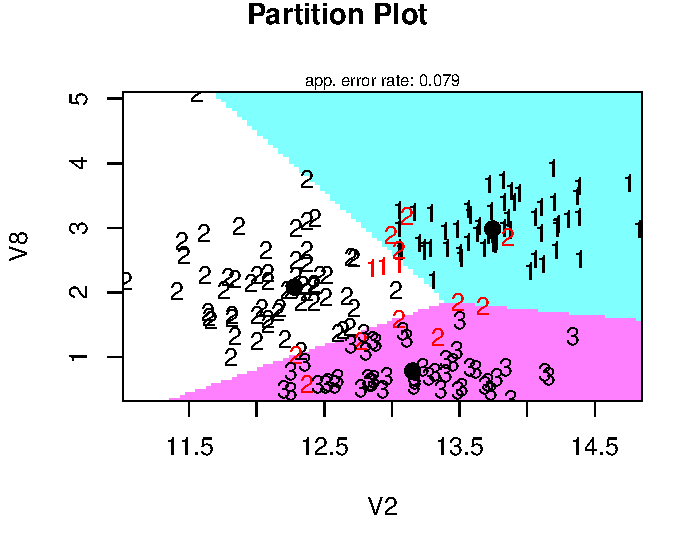
\includegraphics[width=\maxwidth]{figure/unnamed-chunk-12} 

}


\begin{kframe}\begin{alltt}
\hlstd{S}\hlopt{$}\hlstd{freq[}\hlkwd{which.max}\hlstd{(S}\hlopt{$}\hlstd{spec)]}   \hlcom{# czestotliwosc, dla ktorej osiagane }
\end{alltt}
\begin{verbatim}
## [1] 0.1562
\end{verbatim}
\begin{alltt}
                            \hlcom{# jest maksimum gestosci}
\hlnum{1}\hlopt{/}\hlstd{(S}\hlopt{$}\hlstd{freq[}\hlkwd{order}\hlstd{(}\hlopt{-}\hlstd{S}\hlopt{$}\hlstd{spec)[}\hlnum{1}\hlopt{:}\hlnum{2}\hlstd{]])}   \hlcom{# interesuja nas okresy, czyli jeden nad }
\end{alltt}
\begin{verbatim}
## [1] 6.40 1.28
\end{verbatim}
\begin{alltt}
                                  \hlcom{# czestotliwosc, szukamy dwoch }
                                  \hlcom{# najwiekszych wartosci}
                                  \hlcom{# dwa istotne okresy to to powyzej}
\hlkwd{c}\hlstd{(}\hlnum{2}\hlopt{*}\hlstd{pi,}\hlnum{2}\hlopt{/}\hlnum{5}\hlopt{*}\hlstd{pi)}   \hlcom{# a teoretycznie powinnismy dostac to}
\end{alltt}
\begin{verbatim}
## [1] 6.283 1.257
\end{verbatim}
\begin{alltt}
\hlcom{# periodogram: dlaczego na osi x jest od zera do 50? }
\hlcom{# odp: po�owa czestotliwosci, kt�re bralismy}
\hlcom{# widzimy tu dwa maksima}

\hlcom{# zad.2}

\hlkwd{data}\hlstd{(co2)}
\hlkwd{plot}\hlstd{(co2)}
\end{alltt}
\end{kframe}

{\centering \includegraphics[width=\maxwidth]{figure/unnamed-chunk-13} 

}


\begin{kframe}\begin{alltt}
\hlcom{# szereg z trendem i okresowy}

\hlstd{cod} \hlkwb{<-} \hlkwd{diff}\hlstd{(co2)}
\hlkwd{plot}\hlstd{(cod)}   \hlcom{# pozbylismy sie trendu, a okresowosc zostala}
\end{alltt}
\end{kframe}

{\centering \includegraphics[width=\maxwidth]{figure/unnamed-chunk-14} 

}


\begin{kframe}\begin{alltt}
\hlstd{sp} \hlkwb{<-} \hlkwd{spectrum}\hlstd{(co2)}       \hlcom{# maksimum w jedynce i dwojce}
\end{alltt}
\end{kframe}

{\centering \includegraphics[width=\maxwidth]{figure/unnamed-chunk-15} 

}


\begin{kframe}\begin{alltt}
\hlstd{sp.diff} \hlkwb{<-} \hlkwd{spectrum}\hlstd{(cod)}  \hlcom{# maksima zostaja, ale pozbylismy sie trendu, ktory moglby nam przeszkodzic przy estymacji czesci sezonewej}
\end{alltt}
\end{kframe}

{\centering \includegraphics[width=\maxwidth]{figure/unnamed-chunk-16} 

}


\begin{kframe}\begin{alltt}
\hlcom{# ta niebieska kreska to przedzial ufnosci, niekoniecznie symetryczny, }
\hlcom{# tam gdzie kropka to srodek}

\hlcom{# jak to interpretowac? maksimum rowne 1? to okres 1/1, czyli 1, ale czego? }
\hlcom{# jakiej jednostki? 1 rok! dlatego konczy sie na 6, bo wtedy okres to 1/6, }
\hlcom{# czyli dwa miesiace, a czesciej juz sie nie da}

\hlkwd{cpgram}\hlstd{(cod)}
\end{alltt}
\end{kframe}

{\centering \includegraphics[width=\maxwidth]{figure/unnamed-chunk-17} 

}


\begin{kframe}\begin{alltt}
\hlcom{# dystrybuanta spektralna (dwa skoki, czyli mamy dwie skladowe okresowe }
\hlcom{# (najprawdopodobniej)}
\hlcom{# pasek na srodku to pasy ufnosci dla hipotezy o bialym szumie }
\hlcom{# (czyli sprawdzamy, czy jest to bialy szum: tak, jesli caly wykres miesci}
\hlcom{# sie w niebieskich paskach)}

\hlcom{# istotne czestotliwosci (w latach):}
\hlstd{sp.diff}\hlopt{$}\hlstd{freq[}\hlkwd{order}\hlstd{(}\hlopt{-}\hlstd{sp.diff}\hlopt{$}\hlstd{spec)[}\hlnum{1}\hlopt{:}\hlnum{2}\hlstd{]]}
\end{alltt}
\begin{verbatim}
## [1] 1 2
\end{verbatim}
\begin{alltt}
\hlcom{# istotne okresy:}
\hlnum{1}\hlopt{/}\hlstd{sp.diff}\hlopt{$}\hlstd{freq[}\hlkwd{order}\hlstd{(}\hlopt{-}\hlstd{sp.diff}\hlopt{$}\hlstd{spec)[}\hlnum{1}\hlopt{:}\hlnum{2}\hlstd{]]}
\end{alltt}
\begin{verbatim}
## [1] 1.0 0.5
\end{verbatim}
\begin{alltt}
\hlstd{d} \hlkwb{<-} \hlkwd{decompose}\hlstd{(co2)}
\hlkwd{plot}\hlstd{(d)}
\end{alltt}
\end{kframe}

{\centering \includegraphics[width=\maxwidth]{figure/unnamed-chunk-18} 

}


\begin{kframe}\begin{alltt}
\hlcom{# robi dekompozycje na czesc sezonowa, trend, czesc losowa i takie tam}

\hlcom{# zajmijmy sie skladowa sezonowa:}

\hlstd{sp.sez} \hlkwb{<-} \hlkwd{spectrum}\hlstd{(d}\hlopt{$}\hlstd{seasonal)}
\end{alltt}
\end{kframe}

{\centering \includegraphics[width=\maxwidth]{figure/unnamed-chunk-19} 

}


\begin{kframe}\begin{alltt}
\hlkwd{cpgram}\hlstd{(d}\hlopt{$}\hlstd{seasonal)}
\end{alltt}
\end{kframe}

{\centering \includegraphics[width=\maxwidth]{figure/unnamed-chunk-110} 

}


\begin{kframe}\begin{alltt}
\hlstd{sp.sez}\hlopt{$}\hlstd{freq[}\hlkwd{order}\hlstd{(}\hlopt{-}\hlstd{sp.sez}\hlopt{$}\hlstd{spec)[}\hlnum{1}\hlstd{]]}   \hlcom{# czyli jeden rok (co 12 obserwacji)}
\end{alltt}
\begin{verbatim}
## [1] 1
\end{verbatim}
\begin{alltt}
\hlcom{# mamy trzy skladowe okresowe -> chcemy znalezc odpowiadajace im }
\hlcom{#                                czestotliwosci}

\hlcom{# uwaga! szukamy maksimum lokalnego!}

\hlstd{loc.max.coor} \hlkwb{<-} \hlkwa{function}\hlstd{(}\hlkwc{x}\hlstd{) \{}

   \hlstd{n} \hlkwb{<-} \hlkwd{length}\hlstd{(x)}
   \hlstd{Znak} \hlkwb{<-} \hlkwd{diff}\hlstd{(x)}\hlopt{*}\hlkwd{Lag}\hlstd{(}\hlkwd{diff}\hlstd{(x))}
   \hlstd{ex_indices} \hlkwb{<-} \hlkwd{c}\hlstd{(}\hlnum{1}\hlstd{,}\hlkwd{which}\hlstd{(Znak}\hlopt{<}\hlnum{0} \hlopt{&} \hlkwd{diff}\hlstd{(x)}\hlopt{<}\hlnum{0} \hlstd{), n)}   \hlcom{# maksima + brzegi}
   \hlkwd{return} \hlstd{(ex_indices)}
\hlstd{\}}

\hlkwd{loc.max.coor}\hlstd{(}\hlkwd{c}\hlstd{(}\hlnum{0}\hlstd{,}\hlnum{3}\hlstd{,}\hlnum{2}\hlstd{,}\hlnum{6}\hlstd{,}\hlnum{0}\hlstd{,}\hlopt{-}\hlnum{1}\hlstd{,}\hlnum{9}\hlstd{,}\hlnum{10}\hlstd{,}\hlnum{1}\hlstd{))}  \hlcom{# maly test na tej funkcji -> }
\end{alltt}
\begin{verbatim}
## [1] 1 2 4 8 9
\end{verbatim}
\begin{alltt}
                                      \hlcom{# rzeczywiscie zwraca maksima i brzegi}

\hlstd{ist.czest} \hlkwb{<-} \hlstd{sp.diff}\hlopt{$}\hlstd{freq[}\hlkwd{loc.max.coor}\hlstd{(sp.diff}\hlopt{$}\hlstd{spec)]}
\hlcom{# istotne czestotliwosci}

\hlstd{ist.czest[}\hlkwd{order}\hlstd{(}\hlopt{-}\hlstd{sp.diff}\hlopt{$}\hlstd{spec[}\hlkwd{loc.max.coor}\hlstd{(sp.diff}\hlopt{$}\hlstd{spec)])]}
\end{alltt}
\begin{verbatim}
##  [1] 1.000 2.000 1.075 3.000 4.000 1.925 5.100 3.825 5.750 3.875 5.275
## [12] 5.550 2.175 5.425 5.700 2.875 2.650 4.050 2.225 5.475 5.000 5.350
## [23] 3.200 4.100 2.475 4.875 5.625 4.425 4.825 5.900 3.950 2.750 4.250
## [34] 4.300 0.275 2.575 1.800 2.825 3.550 4.650 2.700 3.300 4.550 5.800
## [45] 1.750 3.650 5.975 1.275 3.475 1.225 1.375 3.425 4.175 0.675 1.575
## [56] 0.775 5.150 2.350 4.775 3.350 1.525 4.700 2.425 3.075 1.650 3.750
## [67] 0.175 0.725 0.450 0.100 3.700 0.325 0.025 0.400 0.500 0.575 4.500
## [78] 6.000
\end{verbatim}
\begin{alltt}
\hlcom{# posortowane istotne czestotliwosci}

\hlcom{# jeszcze raz:}

\hlkwd{plot}\hlstd{(d)}
\end{alltt}
\end{kframe}

{\centering \includegraphics[width=\maxwidth]{figure/unnamed-chunk-111} 

}


\begin{kframe}\begin{alltt}
\hlcom{# czemu sa braki danych? bo byla srednia ruchoma, wiec czesc danych tracimy}
\hlcom{# dlaczego czesc sezonowa jest dluzsza mimo, ze braki danych? bo obserwacje }
\hlcom{# sa doliczane zgodnie z sezonowoscia }

\hlcom{# zajmiemy sie czescia losowa:}

\hlstd{sp.rand} \hlkwb{<-} \hlkwd{spectrum}\hlstd{(}\hlkwd{window}\hlstd{(d}\hlopt{$}\hlstd{random,}\hlkwc{start}\hlstd{=}\hlkwd{c}\hlstd{(}\hlnum{1959}\hlstd{,}\hlnum{7}\hlstd{),}\hlkwc{end}\hlstd{=}\hlkwd{c}\hlstd{(}\hlnum{1997}\hlstd{,}\hlnum{6}\hlstd{)))}
\end{alltt}
\end{kframe}

{\centering \includegraphics[width=\maxwidth]{figure/unnamed-chunk-112} 

}


\begin{kframe}\begin{alltt}
\hlkwd{cpgram}\hlstd{(d}\hlopt{$}\hlstd{random)}  \hlcom{# to nie jest bialy szum, a raczej powienien byc}
\end{alltt}
\end{kframe}

{\centering \includegraphics[width=\maxwidth]{figure/unnamed-chunk-113} 

}


\begin{kframe}\begin{alltt}
                  \hlcom{# ale to jeszcze nie koniec swiata, byc moze mozemy }
                  \hlcom{# dopasowac do tego jakis model arma}

\hlcom{# predykcja kolejnych 50 elementow:}

\hlstd{m} \hlkwb{<-} \hlkwd{HoltWinters}\hlstd{(co2,}\hlkwc{seasonal}\hlstd{=}\hlstr{"additive"}\hlstd{)}
\hlstd{m}\hlopt{$}\hlstd{coefficients}
\end{alltt}
\begin{verbatim}
##        a        b       s1       s2       s3       s4       s5       s6 
## 364.7616   0.1247   0.2215   0.9553   1.5985   2.8758   3.2820   2.4407 
##       s7       s8       s9      s10      s11      s12 
##   0.8969  -1.3796  -3.4112  -3.2570  -1.9135  -0.5844
\end{verbatim}
\begin{alltt}
\hlcom{# X_\{12k+i\}=a+b(12k+2)+si}
\hlcom{# s odpowiada za sezonowosc, zas a i b za trend }

\hlcom{# predykcja:}

\hlstd{p} \hlkwb{<-} \hlkwd{predict}\hlstd{(m,}\hlkwc{n.ahead}\hlstd{=}\hlnum{50}\hlstd{,}\hlkwc{prediction.interval}\hlstd{=}\hlnum{TRUE}\hlstd{)}
\hlkwd{plot}\hlstd{(m,p)}   \hlcom{# ladnie :D}
\end{alltt}
\end{kframe}

{\centering \includegraphics[width=\maxwidth]{figure/unnamed-chunk-114} 

}


\begin{kframe}\begin{alltt}
\hlcom{# a teraz bez czesci sezonowej (parametr gamma za to odpowiada):}

\hlstd{m} \hlkwb{<-} \hlkwd{HoltWinters}\hlstd{(co2,}\hlkwc{seasonal}\hlstd{=}\hlstr{"additive"}\hlstd{,}\hlkwc{gamma}\hlstd{=}\hlnum{FALSE}\hlstd{)}
\hlstd{p} \hlkwb{<-} \hlkwd{predict}\hlstd{(m,}\hlkwc{n.ahead}\hlstd{=}\hlnum{50}\hlstd{,}\hlkwc{prediction.interval}\hlstd{=}\hlnum{TRUE}\hlstd{)}
\hlkwd{plot}\hlstd{(m,p)}  \hlcom{# tragiczna predykcja, czyli ta czesc sezonowa }
\end{alltt}
\end{kframe}

{\centering \includegraphics[width=\maxwidth]{figure/unnamed-chunk-115} 

}


\begin{kframe}\begin{alltt}
           \hlcom{# byla rzeczywiscie potrzebna}

\hlcom{# zad.3}

\hlstd{n} \hlkwb{<-} \hlnum{60}
\hlstd{eps} \hlkwb{<-} \hlkwd{rnorm}\hlstd{(n)}
\hlstd{x} \hlkwb{<-} \hlkwd{numeric}\hlstd{(n)}
\hlstd{y} \hlkwb{<-} \hlkwd{numeric}\hlstd{(n)}

\hlcom{# w przod:}

\hlstd{x[}\hlnum{1}\hlstd{]} \hlkwb{<-} \hlnum{0}
\hlkwa{for}\hlstd{(i} \hlkwa{in} \hlnum{2}\hlopt{:}\hlstd{n)\{}
   \hlstd{x[i]} \hlkwb{<-} \hlnum{2}\hlopt{*}\hlstd{x[i}\hlopt{-}\hlnum{1}\hlstd{]} \hlopt{+} \hlstd{eps[i]}
\hlstd{\}}

\hlcom{# w tyl:}

\hlstd{y[}\hlnum{60}\hlstd{]} \hlkwb{<-} \hlnum{0}
\hlkwa{for}\hlstd{(i} \hlkwa{in} \hlstd{n}\hlopt{:}\hlnum{2}\hlstd{)\{}
   \hlstd{y[i}\hlopt{-}\hlnum{1}\hlstd{]} \hlkwb{<-} \hlstd{(y[i]}\hlopt{-}\hlstd{eps[i])}\hlopt{/}\hlnum{2}
\hlstd{\}}

\hlkwd{plot}\hlstd{(x)}
\end{alltt}
\end{kframe}

{\centering \includegraphics[width=\maxwidth]{figure/unnamed-chunk-116} 

}


\begin{kframe}\begin{alltt}
\hlkwd{plot}\hlstd{(y)}
\end{alltt}
\end{kframe}

{\centering \includegraphics[width=\maxwidth]{figure/unnamed-chunk-117} 

}


\begin{kframe}\begin{alltt}
\hlcom{# r�wne}

\hlstd{x[}\hlnum{1}\hlstd{]} \hlkwb{<-} \hlstd{y[}\hlnum{1}\hlstd{]}
\hlkwa{for}\hlstd{(i} \hlkwa{in} \hlnum{2}\hlopt{:}\hlstd{n)\{}
   \hlstd{x[i]} \hlkwb{<-} \hlnum{2}\hlopt{*}\hlstd{x[i}\hlopt{-}\hlnum{1}\hlstd{]} \hlopt{+} \hlstd{eps[i]}
\hlstd{\}}

\hlkwd{plot}\hlstd{(x)}
\end{alltt}
\end{kframe}

{\centering \includegraphics[width=\maxwidth]{figure/unnamed-chunk-118} 

}


\begin{kframe}\begin{alltt}
\hlcom{# powinny byc sobie rowne, wiec skad sie bierze roznica? }
\hlcom{# odp: z bledow numerycznych}
\end{alltt}
\end{kframe}
\end{knitrout}
\end{document}
